\chapter{Sistema de Informação Geográfico}
\label{cap:sig}

\section{Introdução}

O termo Sistemas de Informação Geográfico (SIG) é aplicado para sistemas que realizam o tratamento computacional de dados geográficos. A principal diferença de um SIG para um sistema de informação convencional é sua capacidade de armazenar tanto os atributos descritivos como as geometrias dos diferentes tipos de dados geográficos \cite{camara}.

O SIG é usado frequentemente em projetos e pesquisas ambientais e urbanas, análise de mercado, monitoramento de recursos naturais, e também por outros profissionais cujo trabalho se baseia em mapas, possibilitando uma visão geral de seu ambiente de trabalho, em que todas as informações de uma base determinada estão ao seu alcance. Este trabalho é possível por meio do georreferenciamento da geometria e os atributos dos dados, ou seja, a localização na superfície terrestre e representados em uma projeção cartográfica \cite{websisbra}.

Em \citeonline{queirozferreira}, é apresentada as principais características de um SIG:

\begin{itemize}
\item Inserir e integrar, em uma única base de dados, informações espaciais provenientes de meio físico-biótico, de dados censitários, de cadastros urbano e rural, e outras fontes de dados como imagens de satélite, e  Sistema de Posicionamento Global (GPS);
\item Oferecer mecanismos para combinar as várias informações, através de algoritmos de manipulação e análise, bem como para consultar, recuperar e visualizar o conteúdo da base de dados geográficos.
\end{itemize}

Nas seções deste capítulo, são abordados os principais conceitos relacionados a função de um SIG, arquitetura de um SIG, integração de arquiteturas SIG, SIG Web, arquitetura de um SIG Web, padrões de desenvolvimento de um SIG, Infraestrutura Nacional de Dados Espaciais (INDE) e \textit{Open Geospatial Consortium} (OGC).

\section{Função de um SIG}

O principal aspecto de um SIG reside na forma de como aplicar e agrupar um conjunto de dados e informações para a solução de um determinado problema. Devido a sua ampla gama de aplicações, que incluem temas como agricultura, cadastro urbanos ou rurais, por exemplo, há pelo menos três grandes maneiras de utilizar um SIG \cite{websisbra}:

\begin{itemize}
\item Produção de mapas;
\item Suporte para análise espacial de fenômenos;
\item Banco de dados geográficos, com funções de armazenamento e recuperação de informação espacial.
\end{itemize}

\newpage

É possível aplicar uma diversidade de soluções em um SIG. As características mais comuns são \cite{zeiler}:

\begin{itemize}
\item Integração do SIG com outras aplicações para execução de análise geográfica e científica. Os dados do SIG precisam estar estruturados e armazenados de modo a permitir o acesso aos dados distribuídos;
\item Arquitetura de informação aberta é essencial, pois facilita a integração de dados geográficos com outros dados;
\item Acesso interativo proporciona os mais sofisticados modelos de dados no apoio às questões e análises;
\item Estrutura de dados adequada ao tipo de análise executada. Tal como uma imagem (representação matricial) ou como conjunto dados em formato vetorial.
\end{itemize}

\section{Arquitetura de um SIG}

A arquitetura de um SIG é composto pelos seguintes componentes: interface, entrada e integração de dados, consulta e análise espacial, visualização e plotagem, e por fim, gerência de dados espaciais.

Cada sistema pode implementar estes componentes de forma distinta, mas todos os subsistemas citados devem estar presentes em um SIG \cite{camara}. A Figura \ref{fig:ArquiteturaSIG} apresenta os componentes de um SIG.

No nível mais próximo ao usuário, a interface homem-máquina define como o sistema é operado e controlado. Esta interface pode ser tanto baseada em ambientes \textit{desktops} ou ambientes que possuam navegação com a Internet. No nível intermediário, um SIG deve ter mecanismos de processamento de dados espaciais. A entrada de dados inclui os mecanismos de conversão de dados. Os algoritmos de consulta e análise espacial incluem as operações topológicas, álgebra de mapas, estatística espacial, modelagem numérica de terreno e processamento de imagens. Os mecanismos de visualização e plotagem, devem oferecer suporte adequado para a apreensão cognitiva dos aspectos relevantes dos dados pesquisado. No nível mais interno do sistema, um sistema de gerência de bancos de dados geográfico oferece armazenamento e recuperação dos dados espaciais e seus atributos \cite{camara}.

\begin{figure}[h]
\centering
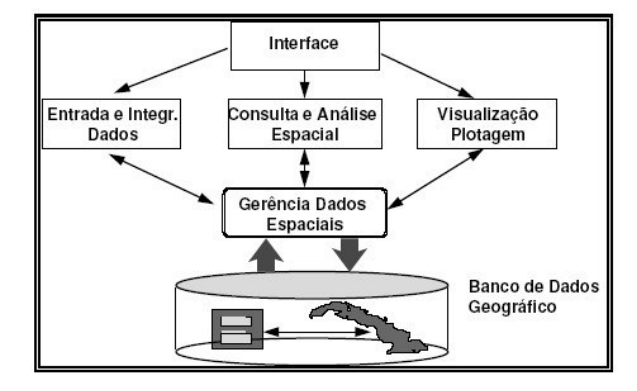
\includegraphics[width=0.65\textwidth]{./img/cap_III/1-ArquiteturaSIG}
\caption{Componentes de um SIG \cite{camara}.}
\label{fig:ArquiteturaSIG}
\end{figure}

Do ponto de vista da aplicação, o uso de um SIG implica em escolher as representações computacionais mais adequadas para capturar a semântica de seu domínio de aplicação. Do ponto de vista da tecnologia, desenvolver um SIG significa oferecer o conjunto mais amplo possível de estruturas de dados e algoritmos capazes de representar a grande diversidade de concepções do espaço \cite{camara}.

\subsection{Modelos de Arquiteturas SIG}

Existem duas principais integrações na arquitetura de um SIG: arquitetura dual e arquitetura integrada. Ambas são definidas a partir da integração entre SIGs e SGBDs \cite{queirozferreira}.

A arquitetura dual representada pela Figura \ref{fig:ArquiteturaDual}, armazena os dados espaciais separadamente dos dados convencionais, ou seja, os dados convencionais são armazenados em um SGBD relacional e os dados espaciais são armazenados em arquivos com formato proprietário. Essa arquitetura ocasiona vários problemas \cite{queirozferreira}:

\begin{itemize}
\item Dificuldade no controle e manipulação dos componentes espaciais;
\item Dificuldade em manter a integridade entre o componente espacial e o componente alfanumérico;
\item Separação entre o processamento da parte convencional, realizado pelo SGBD, e o processamento da parte espacial, realizado pelo aplicativo utilizando os arquivos proprietários;
\item Dificuldade de interoperabilidade, já que cada sistema trabalha com arquivos com formato proprietário.
\end{itemize}

\begin{figure}[h]
\centering
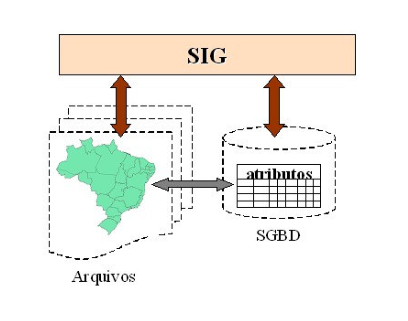
\includegraphics[width=0.50\textwidth]{./img/cap_III/2-ArquiteturaDual}
\caption{Arquitetura dual \cite{queirozferreira}.}
\label{fig:ArquiteturaDual}
\end{figure}

A Figura \ref{fig:ArquiteturaIntegrada} apresenta a arquitetura integrada, que consiste em armazenar todos os dados em um SGBD, ou seja, tanto o componente espacial quanto o alfanumérico. Sua principal vantagem é a utilização dos recursos de um SGBD para controle e manipulação de objetos espaciais, como gerência de transações, controle de integridade, concorrência e linguagens próprias de consulta. Sendo assim, a manutenção de integridade entre o componente espacial e o alfanumérico é feita pelo SGBD \cite{queirozferreira}.

\newpage

\begin{figure}[h]
\centering
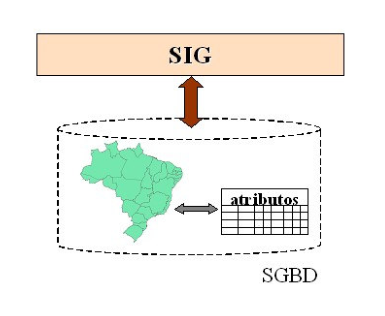
\includegraphics[width=0.50\textwidth]{./img/cap_III/3-ArquiteturaIntegrada}
\caption{Arquitetura integrada \cite{queirozferreira}.}
\label{fig:ArquiteturaIntegrada}
\end{figure}

A arquitetura integrada pode ainda ser subdividida em três outras: baseada em campos longos, em extensões espaciais e combinada \cite{queirozferreira, bancogeo}.

A arquitetura integrada baseada em campos longos utiliza BLOBs (cadeia de bits sem nenhuma semântica adicional) para armazenar os dados espaciais. As desvantagens do uso do BLOB é que ele não possui semântica e não possui métodos de acesso \cite{queirozferreira}.

A arquitetura integrada com extensões espaciais consiste em utilizar extensões espaciais desenvolvidas sobre um Sistema Gerenciador de Banco de Dados Objetos-Relacionais (SGBD-OR). Essa arquitetura permite definir tipos de dados espaciais com operadores específicos e métodos de acesso específicos para dados espaciais, o que a torna muito vantajosa em relação à outra arquitetura. Um exemplo dessa arquitetura é o PostGIS que foi abordado no capítulo anterior deste trabalho \cite{queirozferreira}.

A arquitetura integrada combinada é formada pela combinação das duas anteriores, é utilizada por SIGs que manipulam dados espaciais com geometrias matriciais e vetoriais, as geometrias vetoriais são armazenadas pelos recursos das extensões espaciais e as geometrias matriciais são armazenadas em BLOBs \cite{queirozferreira}.

\section{SIG Web}

A principal característica de um SIG é a capacidade de representar atributos espaciais, além dos atributos convencionais (alfanuméricos). Essa característica adicional permite ilustrar relações, conexões e padrões que não são facilmente visíveis em qualquer conjunto de dados, essa característica torna mais fácil a tomada de decisões nas organizações.

É considerado um SIG Web, qualquer SIG que utiliza tecnologias da Web para interação de dados geográficos, permitindo a visualização dos dados através do uso do \textit{browser}. A utilização do SIG Web permite que o usuário interaja constantemente com o sistema, considerando a facilidade de acesso através de um \textit{browser}, podendo assim, a possibilidade de ser acessado de qualquer dispositivo móvel por exemplo \cite{webgis}.

\newpage

\section{Arquitetura de um SIG Web}

A arquitetura de um SIG Web mais usada é baseada em três camadas: camada de interface, camada de servidor de aplicação e a camada de banco de dados \cite{webgisfuture}. A Figura \ref{fig:ArquiteturaSIGWeb} apresenta a arquitetura de um SIG Web.

\begin{figure}[h]
\centering
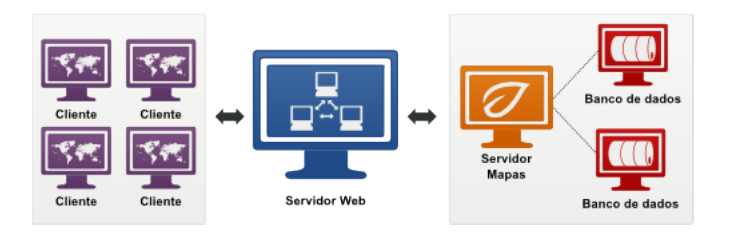
\includegraphics[width=0.65\textwidth]{./img/cap_III/4-ArquiteturaSIGWeb}
\caption{Arquitetura de um SIG Web \cite{websisbra}.}
\label{fig:ArquiteturaSIGWeb}
\end{figure}

\begin{itemize}
\item A Camada de Interface, também conhecida como Camada do Cliente, é a camada responsável por apresentar os dados espaciais no \textit{browser} do usuário. Através da apresentação desses dados, os usuários interagem com os serviços oferecidos pelo SIG Web;
\item A Camada de Servidor de Aplicação é responsável por realizar a comunicação  com as fontes de dados, permitindo o usuário final de analisar e manipular esses dados;
\item A Camada de Banco de Dados faz uso de um banco de dados geográficos para relacionar atributos convencionais e atributos geográficos. Esta camada possui um conjunto de serviços de provedores de dados remotos que são utilizados pelo SIG Web, fazendo que cada banco de dados ofereça um conjunto de interfaces para as aplicações clientes fazerem uso dos dados remotamente.
\end{itemize}

Um SIG Web pode ser desenvolvido a partir de um modelo de arquitetura cliente-servidor, do tipo \textit{thin client} ou \textit{thick client}. O modelo  \textit{thin client}, representado na Figura \ref{fig:ArquiteturaThinClient}, o cliente tem acesso ao servidor somente através da interface de interação para obter as informações. Todo o processamento da aplicação é feito no lado do servidor, que, geralmente, é um computador com maiores recursos computacionais do que o do cliente, de forma a centralizar os recursos \cite{websisbra}.

\begin{figure}[h]
\centering
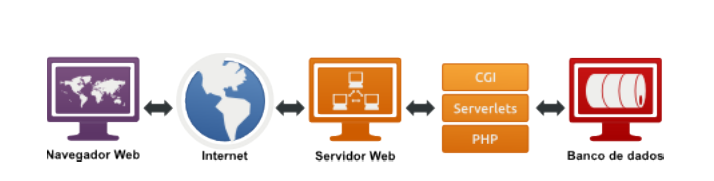
\includegraphics[width=0.70\textwidth]{./img/cap_III/5-ArquiteturaThinClient}
\caption{Modelo de arquitetura \textit{thin client} \cite{websisbra}.}
\label{fig:ArquiteturaThinClient}
\end{figure}

Algumas vantagens no uso desse tipo de arquitetura são:

\begin{itemize}
\item Software centralizado;
\item Facilidade de manutenção;
\item Facilidade de atualização;
\item Controle de acesso simples.
\end{itemize}

Algumas das desvantagens são:

\begin{itemize}
\item Pode ter um tempo de resposta longo;
\item Dados vetoriais não são renderizados no lado do cliente sem que haja a necessidade de ter que instalar algum \textit{plugin} adicional;
\item Grande volume de dados devido a taxa constante de transmissão;
\item Processamento pelo servidor a toda tarefa requisitada, até ações mais simples como: \textit{zoom}, mover e selecionar.
\end{itemize}

A Figura \ref{fig:ArquiteturaThickClient} representa o modelo \textit{thick client}, nesse modelo parte do processamento da aplicação que é executada pelo cliente. Diferente de um \textit{thin client}, esse modelo processa o maior número de informações na camada do cliente, e passa ao servidor somente dados necessários para comunicação e o armazenamento de arquivos. Os navegadores de Internet tem papel fundamental nesse tipo de arquitetura. São clientes leves, capazes de exibir o conteúdo e oferecem suporte a tecnologias que possibilitam a interação com o usuário, como Javascript ou através da adição de \textit{plugins} ou \textit{applets} \cite{websisbra}.

Algumas vantagens no uso desse tipo de arquitetura são:

\begin{itemize}
\item Redução na carga no servidor, usando processamento no cliente;
\item Redução no tráfego da rede, pois os dados podem ser processados localmente;
\item Fácil controle de tarefas simples por parte do cliente (\textit{zoom}, mover, selecionar);
\item Fácil manipulação de mapas vetoriais.
\end{itemize}

Algumas das desvantagens são:

\begin{itemize}
\item Instalação de plugins ou applets;
\item Computador do cliente pode ter um poder de processamento baixo;
\item Carrega, inicialmente, uma quantidade maior de dados.
\end{itemize}

\begin{figure}[h]
\centering

\includegraphics[width=0.75\textwidth]{./img/cap_III/6-ArquiteturaThickClient}
\caption{Modelo de arquitetura \textit{thick client} \cite{websisbra}.}
\label{fig:ArquiteturaThickClient}
\end{figure}

\section{Padrões Para o Desenvolvimento de um SIG}

O emprego de dados geoespaciais, ou seja, dados referenciados à superfície terrestre, é cada vez mais intenso, tanto por usuários públicos quanto privados. O atendimento a essa demanda exige que a produção e a disseminação desses dados sejam realizados de forma ágil. O atual estágio das geotecnologias, como o sensoriamento remoto, o posicionamento por satélites, os sistemas de produção cartográfica, os sistemas de informações geográficos e o acesso à Web (\textit{webmapping}), tem acelerado ainda mais este processo \cite{concar}.

Nesta seção será descrita os principais padrões para desenvolvimento de um SIG.

\subsection{Infraestrutura Nacional de Dados Espaciais}

A Infraestrutura Nacional de Dados Espaciais (INDE) é o conjunto integrado de tecnologias, políticas, mecanismos e procedimentos de coordenação e monitoramento, padrões e acordos, necessário para facilitar e ordenar a geração, o armazenamento, o acesso, o compartilhamento, a disseminação e o uso dos dados geoespaciais de origem federal, estadual, distrital e municipal \cite{inde}.

Dentre as especificações da INDE deve estar presente uma que defina propriadamente a estrutura empregada na aquisição e armazenamento de informações geoespaciais, que permita a disseminação e a disponibilização, otimizando assim o seu compartilhamento, e maximizando a utilidade dos recursos da Tecnologia da Informação, nos diferentes níveis de governo, no setor privado, no terceiro setor, na comunidade acadêmica e na Sociedade como um todo. Para isso, a INDE modelou a estrutura de dados geoespaciais vetoriais utilizando a técnica de modelagem conceitual OMT-G \cite{concar}.

O domínio desse trabalho, SIG Web, não foi especificado pela INDE, logo o modelo conceitual do SIG Web desenvolvido não seguiu nenhuma especificação, foi feito livremente.

\subsection{Open Geospatial Consortium}

\textit{Open Geospatial Consortium} (OGC) é uma organização voluntária internacional de padrões de consenso. Na OGC, mais de 400 organizações comerciais, governamentais, não lucrativas e instituições de pesquisa do mundo todo colaboram num processo de consenso aberto encorajando o desenvolvimento e a implementação de padrões para conteúdo e serviços geomáticos, SIG, processamento e troca de dados. Os padrões estabelecidos pela OGC suportam soluções interoperáveis baseadas na internet e que também são desenvolvidos para trabalhar com informações espaciais complexas e serviços utilizados por diferentes tipos de aplicações \cite{ogc}.

Os padrões atualmente aprovados pela OGC estão agrupados em conjuntos temáticos de serviços de catálogo, serviços de processamento, codificação, serviços de dados, serviços de retrato (imagem) e outros padrões comuns. Em seguida, são descritos os mais importantes \cite{harley, ogc}:

\begin{itemize}
\item \textit{Geographic Markup Language} (GML): Um padrão de codificação baseado em \textit{eXtensible Markup Language} (XML) para informações geográficas desenvolvidas pelo consórcio OGC. A GML foi especificada para o transporte e armazenamento de informação geográfica, incluindo propriedades espaciais e não espaciais das feições geográficas. O objetivo da GML é oferecer um conjunto de regras com as quais um usuário pode definir seu esquema para descrever seus dados. Sua versão 3.0 inclui esquemas que contêm os modelos de geometria, feições e superfícies;
\item \textit{Keyhole Markup Language} (KML): uma notação XML para exibir dados geográficos em um navegador da Terra, como \textit{Google Earth}, \textit{Google Maps}. O KML utiliza uma estrutura de marcadores com elementos e atributos aninhados e se baseia no padrão XML. KML foi desenvolvido para uso com o \textit{Google Earth}, sendo originalmente chamado \textit{Keyhole Earth Viewer}. Foi criado por \textit{Keyhole Inc.} sendo um padrão internacional da OGC, o arquivo KML especifica um conjunto de características (marca local, imagens, polígonos, modelos 3D, descrições textuais, entre outros) para exibição no \textit{Google Earth}, \textit{Maps} e \textit{Mobile}. O KML compartilha algumas das mesmas gramáticas estruturais como GML.

\newpage

\item \textit{Web Map Service} (WMS): é um padrão que fornece uma interface \textit{Hypertext Transfer Protocol} (HTTP) simples para solicitar imagens de mapas georreferenciadas de um ou mais bancos de dados geoespaciais distribuídos. A solicitação WMS define as camadas geográfica(s) e área de interesse a ser processado. A resposta ao pedido é uma ou mais imagens georreferenciadas do mapa (retornado como JPEG, PNG) que podem ser exibidos em um navegador. A interface também suporta a capacidade para especificar se as imagens retornadas devem ser transparentes ou não para que as camadas de vários servidores possam ser combinadas.
\item \textit{Web Feature Services} (WFS): é um serviço padrão, que fornece uma interface de comunicação que permite interagir com mapas atendidos pelo padrão WMS, por exemplo, editar a imagem oferecida pelo serviço WMS ou analisar a imagem usando critérios geográficos. Para realizar essas operações, utiliza-se GML linguagem derivada do XML, que é o padrão pelo qual são transmitidas as ordens WFS, no entanto, qualquer outro formato vetorial pode ser utilizado. WFS não transacional permite a consulta e recuperação de recursos geográficos. Pelo contrário, \textit{Web Feature Service Transacional} (WFS-T) permite também criar, apagar e atualizar esses recursos de mapas geográficos.
\item \textit{Web Coverage Service} (WCS): define uma interface padrão e operações que permitem o acesso interoperável para dados geoespaciais do tipo “matriz”. O termo “matriz” normalmente refere-se a conteúdos como imagens de satélite, fotos aéreas digitais e dados de elevação digital. Este padrão também possui a definição de operação de transação, onde opcionalmente pode ser implementado por servidores WCS. Esta operação de transação permite ao usuário adicional, modificar e eliminar dados matriciais num servidor WCS. As referências de transação ou operação de solicitação incluem a criação de novo dado matricial ou modificações de um existente, abrangendo todos os metadados necessários para um dado matricial.
\end{itemize}